\documentclass[a4paper,11pt]{article}
\usepackage[a4paper, margin=8em]{geometry}

% usa i pacchetti per la scrittura in italiano
\usepackage[french,italian]{babel}
\usepackage[T1]{fontenc}
\usepackage[utf8]{inputenc}
\frenchspacing 

% usa i pacchetti per la formattazione matematica
\usepackage{amsmath, amssymb, amsthm, amsfonts}

% usa altri pacchetti
\usepackage{gensymb}
\usepackage{hyperref}
\usepackage{standalone}

\usepackage{colortbl}

\usepackage{xstring}
\usepackage{karnaugh-map}

% imposta il titolo
\title{Appunti Sistemi Operativi}
\author{Luca Seggiani}
\date{2025}

% imposta lo stile
% usa helvetica
\usepackage[scaled]{helvet}
% usa palatino
\usepackage{palatino}
% usa un font monospazio guardabile
\usepackage{lmodern}

\renewcommand{\rmdefault}{ppl}
\renewcommand{\sfdefault}{phv}
\renewcommand{\ttdefault}{lmtt}

% circuiti
\usepackage{circuitikz}
\usetikzlibrary{babel}

% testo cerchiato
\newcommand*\circled[1]{\tikz[baseline=(char.base)]{
            \node[shape=circle,draw,inner sep=2pt] (char) {#1};}}

% disponi il titolo
\makeatletter
\renewcommand{\maketitle} {
	\begin{center} 
		\begin{minipage}[t]{.8\textwidth}
			\textsf{\huge\bfseries \@title} 
		\end{minipage}%
		\begin{minipage}[t]{.2\textwidth}
			\raggedleft \vspace{-1.65em}
			\textsf{\small \@author} \vfill
			\textsf{\small \@date}
		\end{minipage}
		\par
	\end{center}

	\thispagestyle{empty}
	\pagestyle{fancy}
}
\makeatother

% disponi teoremi
\usepackage{tcolorbox}
\newtcolorbox[auto counter, number within=section]{theorem}[2][]{%
	colback=blue!10, 
	colframe=blue!40!black, 
	sharp corners=northwest,
	fonttitle=\sffamily\bfseries, 
	title=Teorema~\thetcbcounter: #2, 
	#1
}

% disponi definizioni
\newtcolorbox[auto counter, number within=section]{definition}[2][]{%
	colback=red!10,
	colframe=red!40!black,
	sharp corners=northwest,
	fonttitle=\sffamily\bfseries,
	title=Definizione~\thetcbcounter: #2,
	#1
}

% disponi codice
\usepackage{listings}
\usepackage[table]{xcolor}

\definecolor{codegreen}{rgb}{0,0.6,0}
\definecolor{codegray}{rgb}{0.5,0.5,0.5}
\definecolor{codepurple}{rgb}{0.58,0,0.82}
\definecolor{backcolour}{rgb}{0.95,0.95,0.92}

\lstdefinestyle{codestyle}{
		backgroundcolor=\color{black!5}, 
		commentstyle=\color{codegreen},
		keywordstyle=\bfseries\color{magenta},
		numberstyle=\sffamily\tiny\color{black!60},
		stringstyle=\color{green!50!black},
		basicstyle=\ttfamily\footnotesize,
		breakatwhitespace=false,         
		breaklines=true,                 
		captionpos=b,                    
		keepspaces=true,                 
		numbers=left,                    
		numbersep=5pt,                  
		showspaces=false,                
		showstringspaces=false,
		showtabs=false,                  
		tabsize=2
}

\lstdefinestyle{shellstyle}{
		backgroundcolor=\color{black!5}, 
		basicstyle=\ttfamily\footnotesize\color{black}, 
		commentstyle=\color{black}, 
		keywordstyle=\color{black},
		numberstyle=\color{black!5},
		stringstyle=\color{black}, 
		showspaces=false,
		showstringspaces=false, 
		showtabs=false, 
		tabsize=2, 
		numbers=none, 
		breaklines=true
}


\lstdefinelanguage{assembler}{ 
  keywords={AAA, AAD, AAM, AAS, ADC, ADCB, ADCW, ADCL, ADD, ADDB, ADDW, ADDL, AND, ANDB, ANDW, ANDL,
        ARPL, BOUND, BSF, BSFL, BSFW, BSR, BSRL, BSRW, BSWAP, BT, BTC, BTCB, BTCW, BTCL, BTR, 
        BTRB, BTRW, BTRL, BTS, BTSB, BTSW, BTSL, CALL, CBW, CDQ, CLC, CLD, CLI, CLTS, CMC, CMP,
        CMPB, CMPW, CMPL, CMPS, CMPSB, CMPSD, CMPSW, CMPXCHG, CMPXCHGB, CMPXCHGW, CMPXCHGL,
        CMPXCHG8B, CPUID, CWDE, DAA, DAS, DEC, DECB, DECW, DECL, DIV, DIVB, DIVW, DIVL, ENTER,
        HLT, IDIV, IDIVB, IDIVW, IDIVL, IMUL, IMULB, IMULW, IMULL, IN, INB, INW, INL, INC, INCB,
        INCW, INCL, INS, INSB, INSD, INSW, INT, INT3, INTO, INVD, INVLPG, IRET, IRETD, JA, JAE,
        JB, JBE, JC, JCXZ, JE, JECXZ, JG, JGE, JL, JLE, JMP, JNA, JNAE, JNB, JNBE, JNC, JNE, JNG,
        JNGE, JNL, JNLE, JNO, JNP, JNS, JNZ, JO, JP, JPE, JPO, JS, JZ, LAHF, LAR, LCALL, LDS,
        LEA, LEAVE, LES, LFS, LGDT, LGS, LIDT, LMSW, LOCK, LODSB, LODSD, LODSW, LOOP, LOOPE,
        LOOPNE, LSL, LSS, LTR, MOV, MOVB, MOVW, MOVL, MOVSB, MOVSD, MOVSW, MOVSX, MOVSXB,
        MOVSXW, MOVSXL, MOVZX, MOVZXB, MOVZXW, MOVZXL, MUL, MULB, MULW, MULL, NEG, NEGB, NEGW,
        NEGL, NOP, NOT, NOTB, NOTW, NOTL, OR, ORB, ORW, ORL, OUT, OUTB, OUTW, OUTL, OUTSB, OUTSD,
        OUTSW, POP, POPL, POPW, POPB, POPA, POPAD, POPF, POPFD, PUSH, PUSHL, PUSHW, PUSHB, PUSHA, 
				PUSHAD, PUSHF, PUSHFD, RCL, RCLB, RCLW, MOVSL, MOVSB, MOVSW, STOSL, STOSB, STOSW, LODSB, LODSW,
				LODSL, INSB, INSW, INSL, OUTSB, OUTSL, OUTSW
        RCLL, RCR, RCRB, RCRW, RCRL, RDMSR, RDPMC, RDTSC, REP, REPE, REPNE, RET, ROL, ROLB, ROLW,
        ROLL, ROR, RORB, RORW, RORL, SAHF, SAL, SALB, SALW, SALL, SAR, SARB, SARW, SARL, SBB,
        SBBB, SBBW, SBBL, SCASB, SCASD, SCASW, SETA, SETAE, SETB, SETBE, SETC, SETE, SETG, SETGE,
        SETL, SETLE, SETNA, SETNAE, SETNB, SETNBE, SETNC, SETNE, SETNG, SETNGE, SETNL, SETNLE,
        SETNO, SETNP, SETNS, SETNZ, SETO, SETP, SETPE, SETPO, SETS, SETZ, SGDT, SHL, SHLB, SHLW,
        SHLL, SHLD, SHR, SHRB, SHRW, SHRL, SHRD, SIDT, SLDT, SMSW, STC, STD, STI, STOSB, STOSD,
        STOSW, STR, SUB, SUBB, SUBW, SUBL, TEST, TESTB, TESTW, TESTL, VERR, VERW, WAIT, WBINVD,
        XADD, XADDB, XADDW, XADDL, XCHG, XCHGB, XCHGW, XCHGL, XLAT, XLATB, XOR, XORB, XORW, XORL},
  keywordstyle=\color{blue}\bfseries,
  ndkeywordstyle=\color{darkgray}\bfseries,
  identifierstyle=\color{black},
  sensitive=false,
  comment=[l]{\#},
  morecomment=[s]{/*}{*/},
  commentstyle=\color{purple}\ttfamily,
  stringstyle=\color{red}\ttfamily,
  morestring=[b]',
  morestring=[b]"
}

\lstset{language=assembler, style=codestyle}

% disponi sezioni
\usepackage{titlesec}

\titleformat{\section}
	{\sffamily\Large\bfseries} 
	{\thesection}{1em}{} 
\titleformat{\subsection}
	{\sffamily\large\bfseries}   
	{\thesubsection}{1em}{} 
\titleformat{\subsubsection}
	{\sffamily\normalsize\bfseries} 
	{\thesubsubsection}{1em}{}

% tikz
\usepackage{tikz}

% float
\usepackage{float}

% grafici
\usepackage{pgfplots}
\pgfplotsset{width=10cm,compat=1.9}

% disponi alberi
\usepackage{forest}

\forestset{
	rectstyle/.style={
		for tree={rectangle,draw,font=\large\sffamily}
	},
	roundstyle/.style={
		for tree={circle,draw,font=\large}
	}
}

% disponi algoritmi
\usepackage{algorithm}
\usepackage{algorithmic}
\makeatletter
\renewcommand{\ALG@name}{Algoritmo}
\makeatother

% disponi numeri di pagina
\usepackage{fancyhdr}
\fancyhf{} 
\fancyfoot[L]{\sffamily{\thepage}}

\makeatletter
\fancyhead[L]{\raisebox{1ex}[0pt][0pt]{\sffamily{\@title \ \@date}}} 
\fancyhead[R]{\raisebox{1ex}[0pt][0pt]{\sffamily{\@author}}}
\makeatother

\begin{document}
% sezione (data)
\section{Lezione del 08-10-25}

% stili pagina
\thispagestyle{empty}
\pagestyle{fancy}

% testo
Continuiamo la discussione degli algoritmi di scheduling.

\subsubsection{Algoritmo RR}
L'algoritmo \textbf{RR} (\textit{Round Robin}) è preemptive e non prioritario, e si basa su un meccanismo molto semplice: ad ogni processo viene dato un quanto temporale prefissato, e via preemption si passa al processo successivo quando tale quanto viene esaurito.

Questo lo rende molto efficiente: l'overhead $O_v$ è minimo, quasi al pari di FCFS (leggermente più alto in quanto i cambi di contesto sono più frequenti, uno ogni quanto temporale). 
\par\smallskip

Simuliamo questo algoritmo usando la sequenza di processi richiesti già vista in 6.2.2, e imponendo un quanto temporale di $\Delta T = 20$. La tabella dei tempi di richiesta e esecuzione dei processi sarà:
\begin{table}[H]
	\center \rowcolors{2}{white}{black!10}
	\begin{tabular} { c || c | c }
		\bfseries Processo & \bfseries $\mathbf{T}$ richiesta & \bfseries $\mathbf{C}$ esecuzione \\
		\hline
		$p_0$ & 0 & 10 \\ 
		$p_1$ & 2 & 100 \\ 
		$p_2$ & 4 & 24 \\ 
		$p_3$ & 6 & 16 
	\end{tabular}
\end{table}

\newpage

In questo caso la \textit{timeline} avrà un aspetto del genere:
\begin{center}
	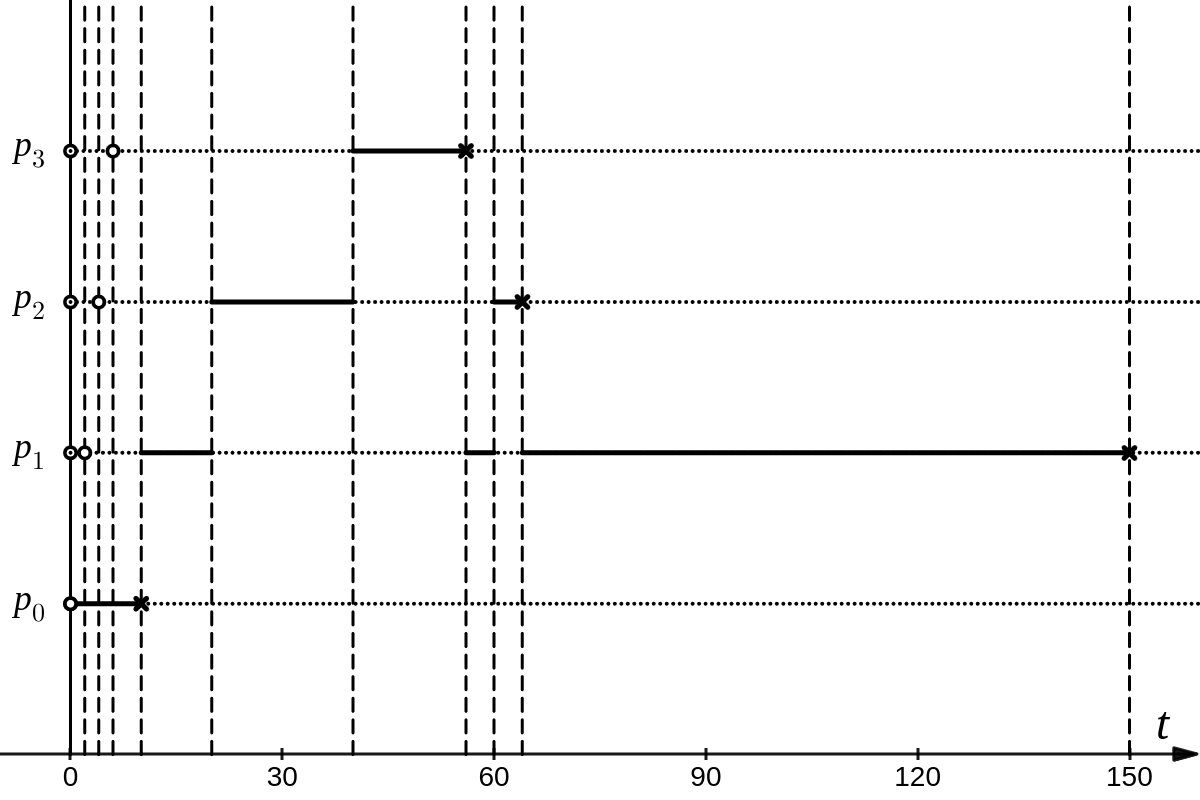
\includegraphics[scale=0.3]{../figures/rr.png}
\end{center}

Vediamo che il tempo medio, calcolato come:
$$
\tilde{t}_a = \frac{{t_a}_0 + {t_a}_1 + {t_a}_2 + {t_a}_3}{4} = \frac{0 + 10 + 20 + 40}{4} = 17.5
$$
sarà più o meno nella norma rispetto a SJR o STRF.

La cosa importante è, come lo era stato per STRF, la \textit{responsività} che l'algoritmo riesce a realizzare: un processo non resta mai in coda pronti per un tempo maggiore al quanto temporale moltiplicato per i processi in esecuzione meno 1.

\par\smallskip

Dal punto di vista implementativo, organizzaremo i quanti temporali sfruttando una componente hardware detta \textbf{timer}: questo è considerato a tutti gli effetti una periferiche, ed invia (dopo un'opportuna configurazione) interruzioni esterne periodiche.
Ogni volta che il processore riceve tale interruzione, mette in esecuzione lo scheduler, che provvede a cambiare il contesto al prossimo processo.
Chiaramente, lo scheduler può comunque essere messo in esecuzione da eventi comuni come la terminazione di processi.

Per realizzare l'esecuzione ciclica si usa una semplice coda pronti dove lo scheduler estreae sempre dalla testa e inserisce sempre in fondo alla coda.

Come abbiamo visto dall'esempio, l'RR rende molto semplice stimare il tempo di attesa: se ci sono $N$ processi in esecuzione, $N - 1$ saranno in coda pronti in qualsiasi momento, quindi un dato processo aspetterà:
$$
T_a = (N - 1)q
$$
dove $q$ è il quanto di tempo.

Chiaramente il $T_a$ diventa troppo grande se ci sono troppi processi.

\subsection{Code multilivello}
Abbiamo quindi discusso i 4 algoritmi di scheduling fondamentali che avevamo introdotto in 6.2.
Ognuno di questi ha pro e contro distinti, ed è più adeguato in una o un altra situazione.

Per questo motivo nei sistemi operativi moderni si preferisce implementare lo scheduling attraverso \textbf{più algoritmi} di scheduling, che gestiscono ognuno la situazione che più conviene.

Un modo elegante di realizzare ciò è mantenere \textbf{più code}, una per ogni algoritmo di scheduling. Sistemi di questo tipo vengono detti \textbf{multilevel queue} o \textit{code multilivello}.

\subsubsection{Code di feedback}
Una variante interessante delle code multilivello è dato dalle \textit{code di feedback}.
Queste nascono per gestire più gerarchie di processi dai requisiti di esecuzione diversi (I/O bound, più interattivi, e CPU bound, più lenti).

In questo caso si prevede una struttura di code, ad esempio come la seguente:
\begin{enumerate}
	\item Coda RR \textit{veloce}, con quanto $\Delta T = 10$;
	\item Coda RR \textit{più lenta}, con quanto $\Delta T = 20$;
	\item Coda FCFS, la più \textit{lenta}.
\end{enumerate}
Le code vengono ordinate per priorità decrescente.

Un processo richiesto viene messo nella coda RR più veloce: se al momento della prima revoca CPU non è riuscito a terminare il suo primo CPU burst, viene spostato nella coda RR più lenta.
La procedura si ripete finché il processo non è giudicato come \textit{non interattivo} e spostato nella coda FCFS.

In questo modo si riescono a sviluppare sistemi che si \textit{"adattano"} in qualche modo a diversi tipi di processi, scegliendo per ognuno la coda (e quindi la politica di schedulazione) più adatta.

\par\smallskip

Facciamo qualche altra considerazione: poniamo che ci sia un processo molto interattivo (magari il processo che si occupa di disegnare l'ambiente grafico) nella prima coda, e un processo CPU bound molto lento (magari un software di calcolo scientifico) in coda FCFS.

Avremo che il processo interattivo farà molti I/O burst (scrittura a video, lettura dati da mouse e tastiera, ecc...) e probabilmente i suoi CPU burst finiranno prima del quanto temporale offerto dalla coda RR.
Sarà in questi istanti che il processo lento potrà entrare in esecuzione nella coda FCFS.

\par\smallskip

L'approccio non è ideale in quanto presenta alcuni difetti:
\begin{itemize}
	\item 
Potrebbero verificarsi casi dove il processo in coda FCFS non riesce ad eseguire di fronte a una grande massa di processi veloci che arrivano in coda RR (\textit{starvation}): per questo motivo gli S/O moderni implementano altri meccanismi, come l'\textit{aging};
	\item
Un'altra problematica è data dal fatto che l'ultima coda è non preemptive: quando un processo dal lungo CPU Burst entra in coda FCFS vi resta finche non ha finito di eseguire, bloccando il resto del sistema. 

Possiamo risolvere questo problema rendendo l'FCFS vagamente \textit{preemptive}: visto che ci sono altre due code prima di essa, possiamo cogliere l'occasione del lancio di un nuovo processo per rimettere in esecuzione lo scheduler. Questo meccanismo non è propriamente necessaria per le prime 2 code in quanto il quanto di tempo è limitato (e quindi prima o poi il nuovo processo viene servito), mentre è fondamentale per la coda FCFS che potrebbe bloccare anche per diverso tempo.
\end{itemize}

Un ultima considerazione che vogliamo fare è se \textit{conviene} riportare i processi dalle code di livello inferiore (più lente) nelle code di livello superiore (più veloci) quando queste si sgombrano: in generale, abbiamo che la letteratura non lo trova particolarmente vantaggioso.
Questo perché un processo che è finito in una coda meno interattiva è probabilmente \textit{meno interattivo}, per cui può godere di CPU burst più lunghi e deve restare nella coda dove si trova.

In caso di \textit{aging}, di contro, questo processo è necessario e più che naturale: spostiamo i processi che sono da molto tempo in code inferiori verso le code superiori per forzarne l'esecuzione.

\end{document}
